\documentclass[11pt]{article}

\usepackage[margin=1in]{geometry}
\usepackage{amsmath,amssymb,amsthm}
\usepackage{graphicx}
\usepackage{hyperref}

\newtheorem*{theorem}{Literature Status Theorem}

\newcommand{\cL}{\mathcal L}
\newcommand{\ellp}{\ell_p}
\newcommand{\ellq}{\ell_q}
\newcommand{\cont}{\mathfrak c}

\title{Literature Status: Infinitely Many Closed Ideals in
  \texorpdfstring{$\mathcal L(\ell_p\oplus\ell_q)$}{L(ell_p plus ell_q)}}
\author{FA/Banach run \texttt{fa\_banach\_001}}
\date{2026-06-14}

\begin{document}
\maketitle

\section*{Packet Status}

This is a \texttt{literature\_already\_answered} packet, not an original
proof from this run.  It records that the infinite-many/cardinality part of
the closed-ideals problem around
\(\cL(\ell_p\oplus\ell_q)\) and \(\cL(\ell_p,\ell_q)\) is already answered in
later literature.

\section*{Original Source}

The source paper is B. Sari, Th. Schlumprecht, N. Tomczak-Jaegermann, and
V. G. Troitsky, \emph{On norm closed ideals in
\(\cL(\ell_p\oplus\ell_q)\)}, arXiv:math/0509414.  Its abstract frames the
next question after the classical \(\ell_p\) and \(c_0\) cases as the problem
of describing all closed ideals of \(\cL(\ell_p\oplus\ell_q)\), equivalently
closed ideals in \(\cL(\ell_p,\ell_q)\) for \(p<q\).  It then proves finite
progress in the range \(1<p<2<q<\infty\).

\begin{figure}[h]
  \centering
  
\includegraphics[width=\linewidth]{figures/open_problem_crop.png}
  \caption{Source question in arXiv:math/0509414, page 1.}
\end{figure}

\section*{Supporting Sources}

The explicit answer source is Th. Schlumprecht and A. Zsak,
\emph{The algebra of bounded linear operators on
\(\ell_p\oplus\ell_q\) has infinitely many closed ideals},
arXiv:1409.3480.  Its abstract says that it solves Pietsch's Problem 5.3.3,
and its introduction restates the problem before proving the main theorem.

The later strengthening is D. Freeman, Th. Schlumprecht, and A. Zsak,
\emph{Banach spaces for which the space of operators has
\(2^{\mathfrak c}\) closed ideals}, arXiv:2006.15415.  Corollary 9 gives
the exact cardinality \(2^{\mathfrak c}\) for the relevant
\(\ell_p\)-sum algebras in the reflexive range.

\begin{figure}[h]
  \centering
  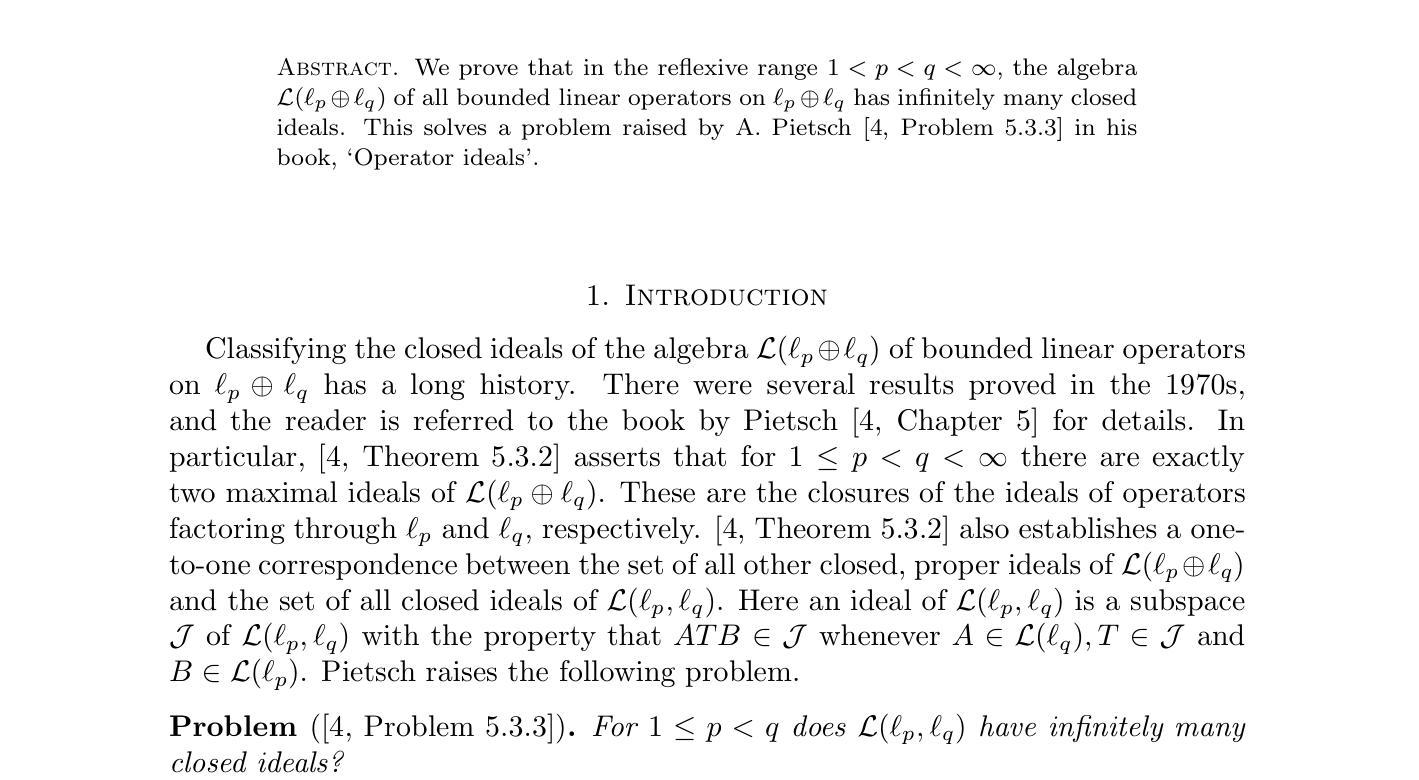
\includegraphics[width=\linewidth]{figures/supporting_pietsch_problem_crop.png}
  \caption{arXiv:1409.3480 explicitly identifies Pietsch's problem and the
  answer claim.}
\end{figure}

\begin{figure}[h]
  \centering
  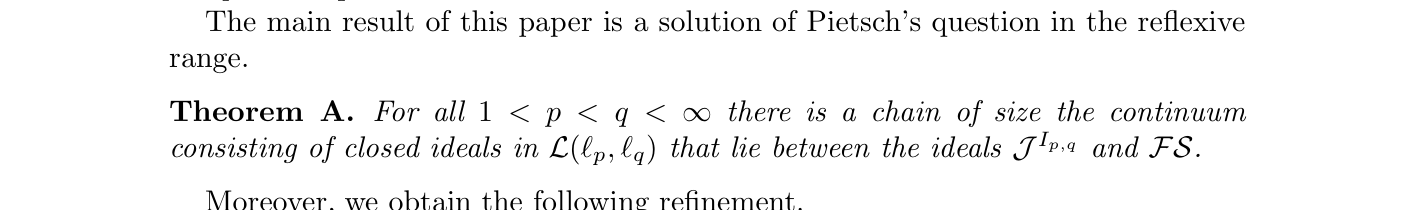
\includegraphics[width=\linewidth]{figures/supporting_main_theorem_crop.png}
  \caption{Theorem A of arXiv:1409.3480 gives a continuum-sized chain in
  \(\cL(\ell_p,\ell_q)\) for \(1<p<q<\infty\).}
\end{figure}

\begin{figure}[h]
  \centering
  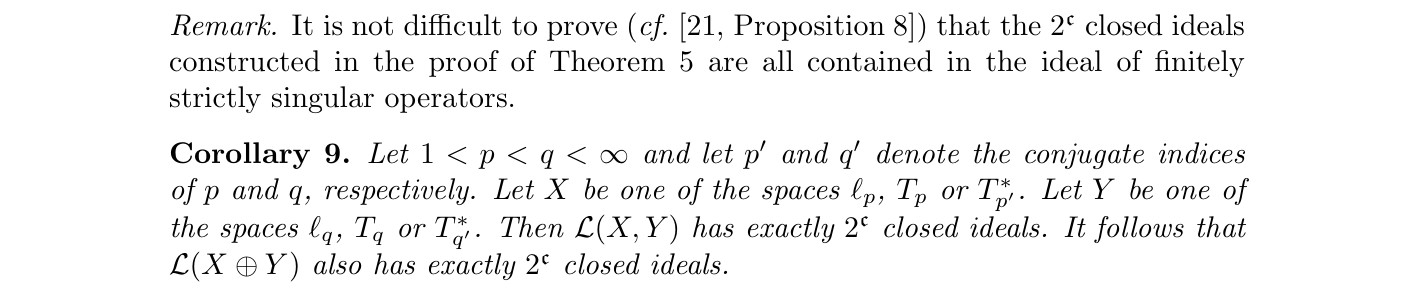
\includegraphics[width=\linewidth]{figures/supporting_exact_cardinality_crop.png}
  \caption{Corollary 9 of arXiv:2006.15415 gives exact cardinality
  \(2^{\mathfrak c}\) for \(\cL(\ell_p\oplus\ell_q)\).}
\end{figure}

\section*{Proof Intuition}

The source problem asks for the closed-ideal structure of
\(\cL(\ell_p\oplus\ell_q)\), and both the 2005 and 2014 papers recall
Pietsch's reduction: apart from the two maximal ideals, proper closed ideals
of the algebra correspond to closed ideals in \(\cL(\ell_p,\ell_q)\).
Therefore a continuum-sized chain in \(\cL(\ell_p,\ell_q)\) immediately
settles the ``infinitely many'' part of the algebra question.  The 2020 paper
then uses a stronger almost-disjoint-family construction to upgrade this from
continuum many to the maximal possible cardinality \(2^{\mathfrak c}\).

\begin{theorem}
For every \(1<p<q<\infty\), Pietsch's question asking whether
\(\cL(\ell_p,\ell_q)\) has infinitely many closed ideals is answered
affirmatively in the later literature.  In fact, there is a chain of
cardinality \(\mathfrak c\) of closed ideals in \(\cL(\ell_p,\ell_q)\), and
the set of closed ideals of \(\cL(\ell_p\oplus\ell_q)\) has cardinality
exactly \(2^{\mathfrak c}\).
\end{theorem}

\begin{proof}
Schlumprecht--Zsak, arXiv:1409.3480, explicitly formulate Pietsch's Problem
5.3.3 as the question whether \(\cL(\ell_p,\ell_q)\) has infinitely many
closed ideals.  The same paper says this is the problem it solves in the
reflexive range.  Its Theorem A proves that for all \(1<p<q<\infty\) there is
a chain of size \(\mathfrak c\) of closed ideals in
\(\cL(\ell_p,\ell_q)\).  This proves the affirmative infinite-many answer.

The connection with the algebra \(\cL(\ell_p\oplus\ell_q)\) is the standard
Pietsch correspondence quoted in the 2005 source and in the 2014 supporting
paper: for \(1\le p<q<\infty\), the algebra has two proper maximal ideals,
and all other proper closed ideals correspond to closed ideals in
\(\cL(\ell_p,\ell_q)\).  Hence the continuum-sized chain gives infinitely
many closed ideals in \(\cL(\ell_p\oplus\ell_q)\).

Freeman--Schlumprecht--Zsak, arXiv:2006.15415, prove a stronger statement.
Their Corollary 9 states that if \(1<p<q<\infty\), then
\(\cL(X,Y)\) has exactly \(2^{\mathfrak c}\) closed ideals for
\(X=\ell_p\) and \(Y=\ell_q\), and consequently
\(\cL(X\oplus Y)\) also has exactly \(2^{\mathfrak c}\) closed ideals.
Taking \(X=\ell_p\) and \(Y=\ell_q\) gives the exact-cardinality assertion for
\(\cL(\ell_p\oplus\ell_q)\).
\end{proof}

\section*{Verification Notes}

\begin{itemize}
  \item Same-paper check: arXiv:math/0509414 proves finite progress but does
  not answer the infinite-many question in the full reflexive range.
  \item Separate-source check: arXiv:1409.3480 is independent and later.  It
  explicitly identifies Pietsch's problem and says it solves it.
  \item Strengthening check: arXiv:2006.15415 is later and gives exact
  cardinality \(2^{\mathfrak c}\), not merely infinitely many ideals.
  \item Local duplicate check: the run registry and indexes were searched for
  \texttt{0509414}, \texttt{1409.3480}, \texttt{2006.15415},
  \texttt{closed ideals}, \texttt{ell\_p oplus ell\_q}, \texttt{Pietsch},
  and \texttt{Schlumprecht Zsak}.
\end{itemize}

\section*{Limitations}

This packet does not claim a full classification of the closed-ideal lattice
of \(\cL(\ell_p\oplus\ell_q)\) or \(\cL(\ell_p,\ell_q)\).  It records only
the infinite-many and exact-cardinality status for \(1<p<q<\infty\).  Endpoint
cases involving \(\ell_1\), \(c_0\), or \(\ell_\infty\) are not included.

\section*{Human Review Recommendation}

Verify the use of Pietsch's correspondence between non-maximal closed ideals
of \(\cL(\ell_p\oplus\ell_q)\) and closed ideals of
\(\cL(\ell_p,\ell_q)\).  If that identification is accepted, the
infinite-many and exact-cardinality conclusions are already literature-known.

\end{document}
